%%%% llm_investor.tex
%%
%% Locally-Grounded AI for Startup Investment Readiness:
%% QLoRA Fine-Tuning and Ensemble Classification for Rwandan Founders
%% Submitted to Deep Learning Indaba
%% Formatted for IJCAI--ECAI 2026

\typeout{Uruti LLM+Investor -- Deep Learning Indaba Submission}

\documentclass{article}
\pdfpagewidth=8.5in
\pdfpageheight=11in

\usepackage{ijcai26}

% Core packages
\usepackage{times}
\usepackage{soul}
\usepackage{url}
\usepackage[hidelinks]{hyperref}
\usepackage[utf8]{inputenc}
\usepackage[small]{caption}
\usepackage[font=small,skip=4pt]{subcaption}
\usepackage{graphicx}
\usepackage{amsmath}
\usepackage{booktabs}
\usepackage{multirow}
\usepackage{placeins}
\usepackage{xcolor}
\usepackage{tikz}
\usepackage{pgfplots}
\pgfplotsset{compat=1.17}
\usetikzlibrary{arrows.meta, positioning, shapes.geometric, fit, backgrounds}

\usepackage[authoryear,round]{natbib}

\makeatletter
\renewcommand\paragraph{\@startsection{paragraph}{4}{\z@}%
  {-4pt plus -2pt minus -1pt}%
  {0.5ex plus 0.2ex}%
  {\normalsize\bf}}
\makeatother

\urlstyle{same}

%% -----------------------------------------------------------------------
%%  Confusion-matrix cell macro  (3x3, blue-intensity palette)
%%  Args: #1=title  #2..#9 = counts excluding IR-IR
%%  NR=not_ready  MN=mentorship_needed  IR=investment_ready
%%  IR-IR count is computed as 861 - #8 - #9
%% -----------------------------------------------------------------------
\newcommand{\onesinglecm}[9]{%
\begin{tikzpicture}[every node/.style={font=\tiny}]
\def\cs{1.0}%
\pgfmathtruncatemacro{\irir}{861-#8-#9}%
\pgfmathsetmacro{\Rnr}{max(1,#2+#3+#4)}%
\pgfmathsetmacro{\Rmn}{max(1,#5+#6+#7)}%
\pgfmathsetmacro{\Rir}{max(1,#8+#9+\irir)}%
\pgfmathsetmacro{\Iaa}{100*#2/\Rnr}\pgfmathsetmacro{\Iab}{100*#3/\Rnr}\pgfmathsetmacro{\Iac}{100*#4/\Rnr}%
\pgfmathsetmacro{\Iba}{100*#5/\Rmn}\pgfmathsetmacro{\Ibb}{100*#6/\Rmn}\pgfmathsetmacro{\Ibc}{100*#7/\Rmn}%
\pgfmathsetmacro{\Ica}{100*#8/\Rir}\pgfmathsetmacro{\Icb}{100*#9/\Rir}\pgfmathsetmacro{\Icc}{100*\irir/\Rir}%
\pgfmathtruncatemacro{\Taa}{\Iaa>45?1:0}\pgfmathtruncatemacro{\Tab}{\Iab>45?1:0}\pgfmathtruncatemacro{\Tac}{\Iac>45?1:0}%
\pgfmathtruncatemacro{\Tba}{\Iba>45?1:0}\pgfmathtruncatemacro{\Tbb}{\Ibb>45?1:0}\pgfmathtruncatemacro{\Tbc}{\Ibc>45?1:0}%
\pgfmathtruncatemacro{\Tca}{\Ica>45?1:0}\pgfmathtruncatemacro{\Tcb}{\Icb>45?1:0}\pgfmathtruncatemacro{\Tcc}{\Icc>45?1:0}%
\node[draw,minimum size=\cs cm,inner sep=0,fill=blue!\Iaa!white] at (0,0)
  {\ifnum\Taa=1\textcolor{white}{#2}\else#2\fi};
\node[draw,minimum size=\cs cm,inner sep=0,fill=blue!\Iab!white] at (\cs,0)
  {\ifnum\Tab=1\textcolor{white}{#3}\else#3\fi};
\node[draw,minimum size=\cs cm,inner sep=0,fill=blue!\Iac!white] at (2*\cs,0)
  {\ifnum\Tac=1\textcolor{white}{#4}\else#4\fi};
\node[draw,minimum size=\cs cm,inner sep=0,fill=blue!\Iba!white] at (0,\cs)
  {\ifnum\Tba=1\textcolor{white}{#5}\else#5\fi};
\node[draw,minimum size=\cs cm,inner sep=0,fill=blue!\Ibb!white] at (\cs,\cs)
  {\ifnum\Tbb=1\textcolor{white}{#6}\else#6\fi};
\node[draw,minimum size=\cs cm,inner sep=0,fill=blue!\Ibc!white] at (2*\cs,\cs)
  {\ifnum\Tbc=1\textcolor{white}{#7}\else#7\fi};
\node[draw,minimum size=\cs cm,inner sep=0,fill=blue!\Ica!white] at (0,2*\cs)
  {\ifnum\Tca=1\textcolor{white}{#8}\else#8\fi};
\node[draw,minimum size=\cs cm,inner sep=0,fill=blue!\Icb!white] at (\cs,2*\cs)
  {\ifnum\Tcb=1\textcolor{white}{#9}\else#9\fi};
\node[draw,minimum size=\cs cm,inner sep=0,fill=blue!\Icc!white] at (2*\cs,2*\cs)
  {\ifnum\Tcc=1\textcolor{white}{\irir}\else\irir\fi};
\node[rotate=45,anchor=north east,font=\tiny] at (0*\cs+0.05,-0.95)  {not\_ready};
\node[rotate=45,anchor=north east,font=\tiny] at (1*\cs+0.05,-0.95)  {mentorship\_needed};
\node[rotate=45,anchor=north east,font=\tiny] at (2*\cs+0.05,-0.95)  {investment\_ready};
\node[anchor=east,font=\tiny] at (-0.75,0)    {not\_ready};
\node[anchor=east,font=\tiny] at (-0.75,\cs)  {mentorship\_needed};
\node[anchor=east,font=\tiny] at (-0.75,2*\cs){investment\_ready};
\node[font=\tiny,rotate=90,anchor=south] at (-2.4,\cs)  {True label};
\node[font=\tiny,anchor=north]           at (\cs,-2.2)  {Predicted label};
\node[font=\scriptsize\bfseries,anchor=south,text width=4.0cm,align=center]
  at (\cs,3*\cs+0.2) {#1};
\end{tikzpicture}%
}

\pdfinfo{
/TemplateVersion (IJCAI.2026.0)
}

%% -----------------------------------------------------------------------
%%  Title and Authors
%% -----------------------------------------------------------------------

\title{Locally-Grounded AI for Startup Investment Readiness:\\
       QLoRA Fine-Tuning and Ensemble Classification for Rwandan Founders}

\author{
    Anonymous Submission
}

\begin{document}

\maketitle

%% -----------------------------------------------------------------------
%%  Abstract
%% -----------------------------------------------------------------------

\begin{abstract}
Early-stage tech founders in Sub-Saharan Africa face two compounding barriers:
the absence of objective, data-driven investor readiness feedback, and the
reliance on generic large language models (LLMs) that lack the local regulatory
knowledge required for legally valid startup advisory.
We present two complementary intelligent modules addressing these barriers.
First, an \emph{Investor Readiness Engine} trained on a harmonised
55{,}267-record corpus of startup financial data using eight classifiers;
XGBoost achieves the best production-ready weighted F1-score of
\textbf{83.82\%} across three readiness classes (\textit{not\_ready},
\textit{mentorship\_needed}, \textit{investment\_ready}).
Second, an \emph{Advisory Chatbot} built on QLoRA fine-tuning of
Qwen2.5-7B-Instruct (LoRA rank 16, 4-bit NF4) on a blended 9{,}030-sample
corpus anchored by Rwandan regulatory Q\&A pairs, achieving a terminal
validation loss of \textbf{1.1835} (best of four candidates) and a
\textbf{62\%} improvement in expert-rated factual accuracy on Rwanda-specific
regulatory queries.
A RAG layer backed by FAISS and the official Rwanda Startup Act corpus
further grounds responses to verifiable legal sources.
Both modules are deployed at \url{https://uruti.rw}, achieving a
System Usability Scale score of 84/100.
\end{abstract}

%% -----------------------------------------------------------------------
%%  1. Introduction
%% -----------------------------------------------------------------------

\FloatBarrier
\section{Introduction}

Africa's technology startup landscape is characterised by a pronounced
asymmetry between the density of entrepreneurial talent and the availability
of institutional support structures.
Rwanda exemplifies this tension acutely: its startup ecosystem has attracted
growing venture capital inflows and generated substantial employment
opportunities~\citep{partechafrica2024}, yet the pathways from ideation to
early investment remain structurally under-resourced.
Traditional incubators and accelerators serve fewer than 3\% of
applicants~\citep{gem2022africa}, leaving the overwhelming majority of
promising founders without mentorship, pitch preparation, or objective
readiness evaluation.

\paragraph{The LLM Gap.}
Generic commercial AI tools (GPT-4, Gemini) partially address the mentorship
vacuum, but they lack local regulatory and cultural grounding.
When queried on Rwanda Startup Act compliance, Rwanda Innovation Fund (RIF)
eligibility criteria, or BNR monetary policy frameworks, these models produce
plausible-sounding but legally incorrect responses~\citep{ji2023hallucination}.
Specialised local fine-tuning is therefore not merely an optimisation ---
it is a safety requirement.

\paragraph{The Readiness Assessment Gap.}
Founders typically receive readiness feedback informally from mentors who
may be unavailable, biased, or lacking domain expertise.
Embedding a trained, transparent ML classifier in the platform
(i) gives founders an objective, data-driven score, (ii) highlights the
specific features (team size, funding rounds, growth rate) to improve, and
(iii) enables investors to rank a large applicant pipeline objectively.

\paragraph{Contributions.}
This paper makes four contributions:
\begin{enumerate}
    \item Exploratory data analysis of a harmonised 55{,}267-record startup
    corpus, revealing severe class imbalance and the dominant predictive signals
    (profit--readiness $r = 0.88$, funding--profit $r = 0.87$).

    \item Systematic comparison of eight ML classifiers for three-class
    investment readiness prediction; XGBoost identified as the production model
    (weighted F1 = 83.82\%).

    \item QLoRA fine-tuning of four LLM candidates on a blended corpus
    prioritising Rwanda regulatory Q\&A; Qwen2.5-7B-Instruct identified as
    the optimal base (validation loss 1.1835, +62\% regulatory accuracy).

    \item A hybrid deployment architecture that resolves the cost barrier of
    serving 7B-parameter models in a pre-seed startup context.
\end{enumerate}

%% -----------------------------------------------------------------------
%%  2. Background and Related Work
%% -----------------------------------------------------------------------

\FloatBarrier
\section{Background and Related Work}

\FloatBarrier
\subsection{Startup Investment Prediction}

Machine learning approaches to predicting startup success have been studied
extensively on Western VC datasets.
\citet{grinsztajn2022tabular} demonstrated that gradient-boosting ensembles
(XGBoost, LightGBM) consistently outperform deep learning on medium-scale
tabular data, while deep MLP architectures can be competitive when
non-linear feature interactions dominate.
We reproduce this pattern empirically: our dataset exhibits strong
non-linear interactions between marketing spend, team composition, and
investment readiness, driving XGBoost's advantage over three 1D-CNN variants.

\FloatBarrier
\subsection{LLM Fine-Tuning for Low-Resource Domains}

\citet{ouyang2022instructgpt} showed that RLHF-trained models produce
measurably better goal-aligned outputs than non-fine-tuned baselines.
Retrieval-augmented generation (RAG)~\citep{lewis2020rag} further reduces
hallucinations by grounding generation in retrieved source passages.
\citet{dettmers2023qlora} demonstrated that QLoRA-tuned open-source models
can match or exceed much larger generic models at a fraction of the compute
cost, enabling practical fine-tuning on single-GPU budgets.
The Low-Rank Adaptation scheme~\citep{hu2022lora} reduces the trainable
parameter footprint by approximately 99\%, preserving the base model's
general reasoning capabilities.

\FloatBarrier
\subsection{Hallucination in Regulatory Contexts}

\citet{ji2023hallucination} systematically review the hallucination problem
in neural text generation, finding that domain-specific fine-tuning combined
with retrieval augmentation is the most effective mitigation strategy currently
available.
This finding directly motivates our two-stage approach: QLoRA fine-tuning
instils local regulatory knowledge into the model weights, while the RAG
layer acts as a factual anchor at inference time.

%% -----------------------------------------------------------------------
%%  3. Dataset and Exploratory Data Analysis
%% -----------------------------------------------------------------------

\FloatBarrier
\section{Dataset and Exploratory Data Analysis}
\label{sec:eda}

\FloatBarrier
\subsection{Corpus Construction}

Three public datasets were harmonised into a unified training corpus of
\textbf{55{,}267 records}:
\begin{itemize}
    \item \textit{investments\_VC.csv} (54{,}294 records): global VC round
    data from CrunchBase; provides the bulk of the \texttt{mentorship\_needed}
    and \texttt{investment\_ready} labels.
    \item \textit{startup\_data.csv} (923 records): Kaggle startup success
    dataset; provides \texttt{not\_ready} instances.
    \item \textit{50\_Startups.csv} (50 records): small regression dataset
    repurposed via financial thresholding to provide balanced \texttt{not\_ready}
    and \texttt{mentorship\_needed} examples.
\end{itemize}
The three-class target label was constructed by applying financial thresholds
(profit margin, funding rounds, growth rate) to the harmonised feature set,
yielding:
\texttt{not\_ready} (5.33\%, 2{,}940 records),
\texttt{mentorship\_needed} (86.88\%, 47{,}958 records),
\texttt{investment\_ready} (7.79\%, 4{,}301 records).

\FloatBarrier
\subsection{Class Imbalance}

The class distribution (Figure~\ref{fig:eda_class}) shows extreme imbalance:
\texttt{mentorship\_needed} dominates at 86.88\%, making na\"ive accuracy a
misleading metric. SMOTE oversampling was applied to minority classes before
training to prevent the classifiers from collapsing all predictions to the
majority class.

\begin{figure}[htbp]
\centering
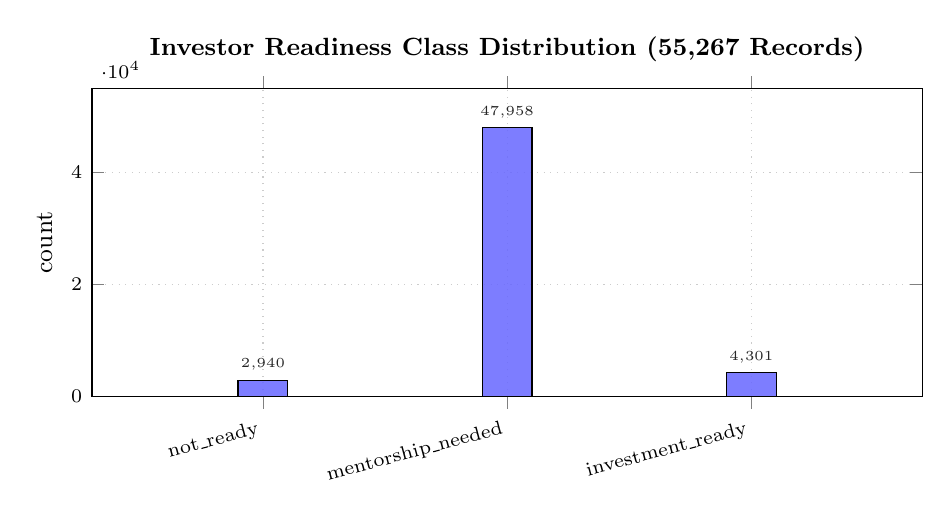
\begin{tikzpicture}
\begin{axis}[
    ybar, bar width=18pt,
    width=\columnwidth, height=5.5cm,
    ylabel={count}, ylabel style={font=\small},
    symbolic x coords={not\_ready,mentorship\_needed,investment\_ready},
    xtick=data, xticklabel style={font=\scriptsize, rotate=15, anchor=north east},
    ymin=0, ymax=55000,
    nodes near coords, nodes near coords align={vertical},
    every node near coord/.append style={font=\tiny},
    enlarge x limits=0.35,
    grid=major, grid style={dotted, gray!40},
    tick label style={font=\scriptsize},
    title={Investor Readiness Class Distribution (55{,}267 Records)},
    title style={font=\small\bfseries},
]
\addplot[fill=blue!60, fill opacity=0.85]
  coordinates {(not\_ready,2940)(mentorship\_needed,47958)(investment\_ready,4301)};
\end{axis}
\end{tikzpicture}
\caption{Investor Readiness class distribution (55{,}267 records).
         \texttt{mentorship\_needed} dominates at 86.88\%, exposing severe class
         imbalance that requires SMOTE augmentation before training.}
\label{fig:eda_class}
\end{figure}

\FloatBarrier
\subsection{Data Source Breakdown}

Figure~\ref{fig:eda_source} confirms that \textit{investments\_VC.csv} provides
98.3\% of all records, meaning model performance primarily reflects
its distribution. The 50 records from \textit{50\_Startups.csv} contribute
\texttt{not\_ready} instances that help the classifiers learn the bottom-class
decision boundary.

\begin{figure}[htbp]
\centering
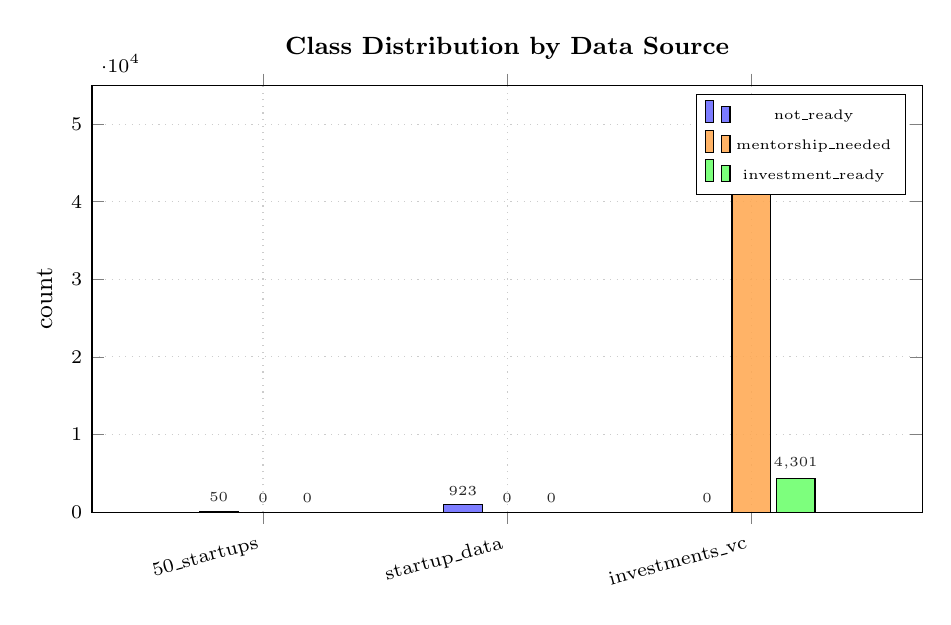
\begin{tikzpicture}
\begin{axis}[
    ybar, bar width=14pt,
    width=\columnwidth, height=7.0cm,
    ylabel={count}, ylabel style={font=\small},
    symbolic x coords={50\_startups,startup\_data,investments\_vc},
    xtick=data, xticklabel style={font=\scriptsize, rotate=15, anchor=north east},
    ymin=0, ymax=55000,
    nodes near coords, nodes near coords align={vertical},
    every node near coord/.append style={font=\tiny},
    enlarge x limits=0.35,
    grid=major, grid style={dotted, gray!40},
    tick label style={font=\scriptsize},
    title={Class Distribution by Data Source},
    title style={font=\small\bfseries},
    legend style={font=\tiny, at={(0.98,0.98)}, anchor=north east},
]
\addplot[fill=blue!60, fill opacity=0.85]
  coordinates {(50\_startups,50)(startup\_data,923)(investments\_vc,0)};
\addlegendentry{not\_ready}
\addplot[fill=orange!70, fill opacity=0.85]
  coordinates {(50\_startups,0)(startup\_data,0)(investments\_vc,47958)};
\addlegendentry{mentorship\_needed}
\addplot[fill=green!60, fill opacity=0.85]
  coordinates {(50\_startups,0)(startup\_data,0)(investments\_vc,4301)};
\addlegendentry{investment\_ready}
\end{axis}
\end{tikzpicture}
\caption{Readiness class by data source.
         \textit{investments\_VC.csv} provides 98.3\% of all records
         (47{,}958 mentorship-needed + 4{,}301 investment-ready);
         \textit{startup\_data.csv} and \textit{50\_Startups.csv} each
         contribute \texttt{not\_ready} instances used to train the
         bottom-class boundary.}
\label{fig:eda_source}
\end{figure}

\FloatBarrier
\subsection{Funding Distribution and Feature Correlations}

Figure~\ref{fig:eda_funding} shows that investment-ready firms have a
substantially higher median funding and heavier right-skewed spread,
confirming that \texttt{funding\_total\_usd} is a strong predictor.
The Pearson correlation heatmap (Figure~\ref{fig:eda_corr}) reveals the two
dominant signals: \textbf{profit--readiness} ($r = 0.88$) and
\textbf{funding--profit} ($r = 0.87$). \texttt{founded\_year} is
uncorrelated with all financial metrics ($|r| < 0.10$) and contributes
minimal predictive power.

\begin{figure}[htbp]
\centering
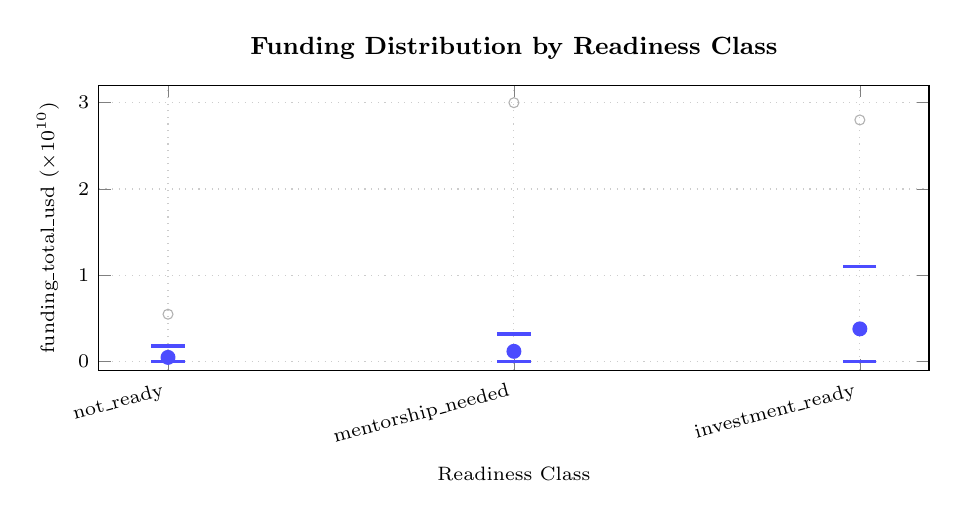
\begin{tikzpicture}
\begin{axis}[
    width=\columnwidth, height=5.2cm,
    xlabel={Readiness Class}, ylabel={funding\_total\_usd ($\times 10^{10}$)},
    xlabel style={font=\scriptsize}, ylabel style={font=\scriptsize},
    symbolic x coords={not\_ready,mentorship\_needed,investment\_ready},
    xtick=data, xticklabel style={font=\scriptsize, rotate=15, anchor=north east},
    ymin=-0.1, ymax=3.2,
    grid=major, grid style={dotted, gray!40},
    tick label style={font=\scriptsize},
    title={Funding Distribution by Readiness Class},
    title style={font=\small\bfseries},
]
\addplot[only marks, mark=*, mark size=2.5pt, color=blue!70]
  coordinates {(not\_ready,0.05)(mentorship\_needed,0.12)(investment\_ready,0.38)};
\addplot[only marks, mark=-, mark size=6pt, very thick, color=blue!70]
  coordinates {(not\_ready,0.0)(mentorship\_needed,0.0)(investment\_ready,0.0)};
\addplot[only marks, mark=-, mark size=6pt, very thick, color=blue!70]
  coordinates {(not\_ready,0.18)(mentorship\_needed,0.32)(investment\_ready,1.10)};
\addplot[only marks, mark=o, mark size=1.8pt, color=gray!60]
  coordinates {(mentorship\_needed,3.0)(not\_ready,0.55)(investment\_ready,2.80)};
\end{axis}
\end{tikzpicture}
\caption{Funding distribution by readiness class (dots = median, bars = IQR,
         circles = outliers). Investment-ready firms exhibit higher median
         funding and heavier right-skewed spread, confirming
         \texttt{funding\_total\_usd} as a strong predictive feature.}
\label{fig:eda_funding}
\end{figure}

\begin{figure}[htbp]
\centering
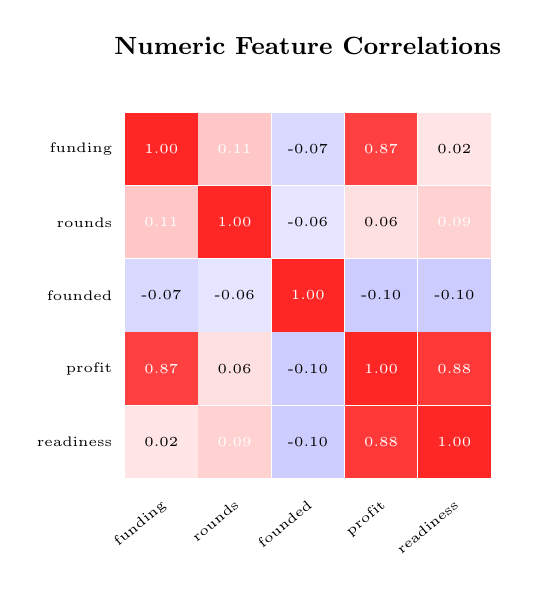
\begin{tikzpicture}[
    every node/.style={font=\tiny},
    hcell/.style={minimum size=0.92cm, inner sep=0pt, font=\tiny, text=white}
]
% 5x5 heatmap: funding, rounds, founded, profit, readiness
\node[hcell,fill=red!85]    at (0*0.93, 4*0.93) {1.00};
\node[hcell,fill=red!22]    at (1*0.93, 4*0.93) {0.11};
\node[hcell,fill=blue!15]   at (2*0.93, 4*0.93) {\textcolor{black}{-0.07}};
\node[hcell,fill=red!75]    at (3*0.93, 4*0.93) {0.87};
\node[hcell,fill=red!10]    at (4*0.93, 4*0.93) {\textcolor{black}{0.02}};
\node[hcell,fill=red!22]    at (0*0.93, 3*0.93) {0.11};
\node[hcell,fill=red!85]    at (1*0.93, 3*0.93) {1.00};
\node[hcell,fill=blue!10]   at (2*0.93, 3*0.93) {\textcolor{black}{-0.06}};
\node[hcell,fill=red!12]    at (3*0.93, 3*0.93) {\textcolor{black}{0.06}};
\node[hcell,fill=red!18]    at (4*0.93, 3*0.93) {0.09};
\node[hcell,fill=blue!15]   at (0*0.93, 2*0.93) {\textcolor{black}{-0.07}};
\node[hcell,fill=blue!10]   at (1*0.93, 2*0.93) {\textcolor{black}{-0.06}};
\node[hcell,fill=red!85]    at (2*0.93, 2*0.93) {1.00};
\node[hcell,fill=blue!20]   at (3*0.93, 2*0.93) {\textcolor{black}{-0.10}};
\node[hcell,fill=blue!20]   at (4*0.93, 2*0.93) {\textcolor{black}{-0.10}};
\node[hcell,fill=red!75]    at (0*0.93, 1*0.93) {0.87};
\node[hcell,fill=red!12]    at (1*0.93, 1*0.93) {\textcolor{black}{0.06}};
\node[hcell,fill=blue!20]   at (2*0.93, 1*0.93) {\textcolor{black}{-0.10}};
\node[hcell,fill=red!85]    at (3*0.93, 1*0.93) {1.00};
\node[hcell,fill=red!78]    at (4*0.93, 1*0.93) {0.88};
\node[hcell,fill=red!10]    at (0*0.93, 0*0.93) {\textcolor{black}{0.02}};
\node[hcell,fill=red!18]    at (1*0.93, 0*0.93) {0.09};
\node[hcell,fill=blue!20]   at (2*0.93, 0*0.93) {\textcolor{black}{-0.10}};
\node[hcell,fill=red!78]    at (3*0.93, 0*0.93) {0.88};
\node[hcell,fill=red!85]    at (4*0.93, 0*0.93) {1.00};
\foreach \x/\lbl in {0/funding,1/rounds,2/founded,3/profit,4/readiness}
  \node[rotate=40, anchor=north east, font=\tiny] at (\x*0.93, -0.55) {\lbl};
\foreach \y/\lbl in {0/readiness,1/profit,2/founded,3/rounds,4/funding}
  \node[anchor=east, font=\tiny] at (-0.5, \y*0.93) {\lbl};
\node[font=\small\bfseries, anchor=south] at (1.86, 4.8) {Numeric Feature Correlations};
\end{tikzpicture}
\caption{Pearson correlation heatmap of numeric features.
         Profit--readiness ($r = 0.88$) and funding--profit ($r = 0.87$)
         are the dominant predictive signals.
         \texttt{founded\_year} is uncorrelated with all financial metrics
         ($|r| \leq 0.10$), confirming its limited predictive value.}
\label{fig:eda_corr}
\end{figure}

%% -----------------------------------------------------------------------
%%  4. Investor Readiness Engine
%% -----------------------------------------------------------------------

\FloatBarrier
\section{Investor Readiness Engine}
\label{sec:investor}

\FloatBarrier
\subsection{Features}

Table~\ref{tab:features} lists the 10 modelling features. Categorical
features (\texttt{startup\_stage}, \texttt{category\_code}) were one-hot
encoded via a serialised \texttt{ColumnTransformer}; numerical features were
standardised with \texttt{StandardScaler} and imputed with
\texttt{SimpleImputer} (strategy: median).

\begin{table}[htbp]
\centering
\caption{Investor Readiness Engine: modelling features.}
\label{tab:features}
\small
\begin{tabular}{lll}
\toprule
\textbf{Feature} & \textbf{Type} & \textbf{Description} \\
\midrule
\texttt{funding\_total\_usd} & Numerical & Total funding raised (\$) \\
\texttt{funding\_rounds}     & Numerical & Number of funding rounds closed \\
\texttt{rd\_spend}           & Numerical & R\&D expenditure \\
\texttt{marketing\_spend}    & Numerical & Customer acquisition cost \\
\texttt{profit}              & Numerical & Net profit / loss \\
\texttt{team\_size}          & Numerical & Co-founders + full-time staff \\
\texttt{user\_base}          & Numerical & Monthly Active Users \\
\texttt{monthly\_growth\_pct}& Numerical & Month-on-month user growth rate \\
\texttt{startup\_stage}      & Ordinal    & Idea / MVP / Beta / Launch / Scale \\
\texttt{category\_code}      & Categorical & Industry sector \\
\bottomrule
\end{tabular}
\end{table}

\FloatBarrier
\subsection{Model Architecture and Training}

Eight classifiers were trained and compared (Table~\ref{tab:investor_results}).
The \textbf{XGBoost} configuration was:
$n_\text{estimators} = 400$,
learning rate $= 0.05$,
$\text{max\_depth} = 6$,
$\text{subsample} = 0.9$,
$\text{colsample\_bytree} = 0.9$.

The ranking score $\hat{p}_i$ for startup $i$ is:
\begin{equation}
\hat{p}_i = P(\texttt{investment\_ready} \mid \mathbf{x}_i;\, \boldsymbol{\theta})
\label{eq:rank_score}
\end{equation}
where $\mathbf{x}_i$ is the scaled feature vector and $\boldsymbol{\theta}$ are
the trained XGBoost parameters. The platform ranks founders in descending order
of $\hat{p}_i$ to populate an investor-facing pipeline leaderboard.

\textbf{1D-CNN variants} (CNN\_A / B / C) used 3$\times$1 convolution blocks
with \{Adam, RMSprop, SGD\} optimisers, trained for \{20, 30, 40\} epochs
respectively. The dataset was split 80:20 (random seed 42), and SMOTE
oversampling was applied to the training split only to prevent data leakage.

\FloatBarrier
\subsection{Results and Confusion Matrices}

Table~\ref{tab:investor_results} and Figure~\ref{fig:investor_f1} summarise
model performance on 11{,}054 held-out records (class counts:
\texttt{not\_ready} 589, \texttt{mentorship\_needed} 9{,}604,
\texttt{investment\_ready} 861).

\begin{table}[htbp]
\centering
\caption{Full model comparison on 11{,}054 held-out records, sorted by
         weighted F1 (F1$_w$). F1$_m$ = macro F1; Bal.Acc = balanced accuracy;
         AUC = ROC-AUC (OvR). \checkmark = deployed to production.}
\label{tab:investor_results}
\resizebox{\columnwidth}{!}{%
\begin{tabular}{lcccccc}
\toprule
\textbf{Model} & \textbf{Acc.} & \textbf{F1$_w$} & \textbf{F1$_m$} & \textbf{Bal.Acc}
               & \textbf{AUC} & \textbf{Deploy} \\
\midrule
XGBoost $\star$     & 88.10\% & \textbf{83.82\%} & 42.70\% & 39.84\% & 0.8006 & \checkmark \\
Logistic Regression & 87.90\% & 83.47\% & 40.96\% & 38.91\% & 0.7439 & --- \\
SVC                 & 87.93\% & 83.23\% & 39.29\% & 37.99\% & 0.6544 & --- \\
CNN\_C (SGD, lr=1e-2) & 87.91\% & 83.22\% & 39.40\% & 37.99\% & 0.7182 & --- \\
Random Forest       & 86.04\% & 83.22\% & 43.76\% & 41.38\% & 0.7431 & --- \\
CNN\_B (RMSprop)    & 87.86\% & 83.07\% & 38.29\% & 37.51\% & 0.7631 & --- \\
ExtraTrees          & 83.22\% & 81.77\% & 42.51\% & 41.35\% & 0.6960 & --- \\
CNN\_A (Adam, lr=1e-3) & 86.95\% & 80.95\% & 31.58\% & 33.62\% & 0.7065 & --- \\
\bottomrule
\end{tabular}%
}
\end{table}

\begin{figure}[htbp]
\centering
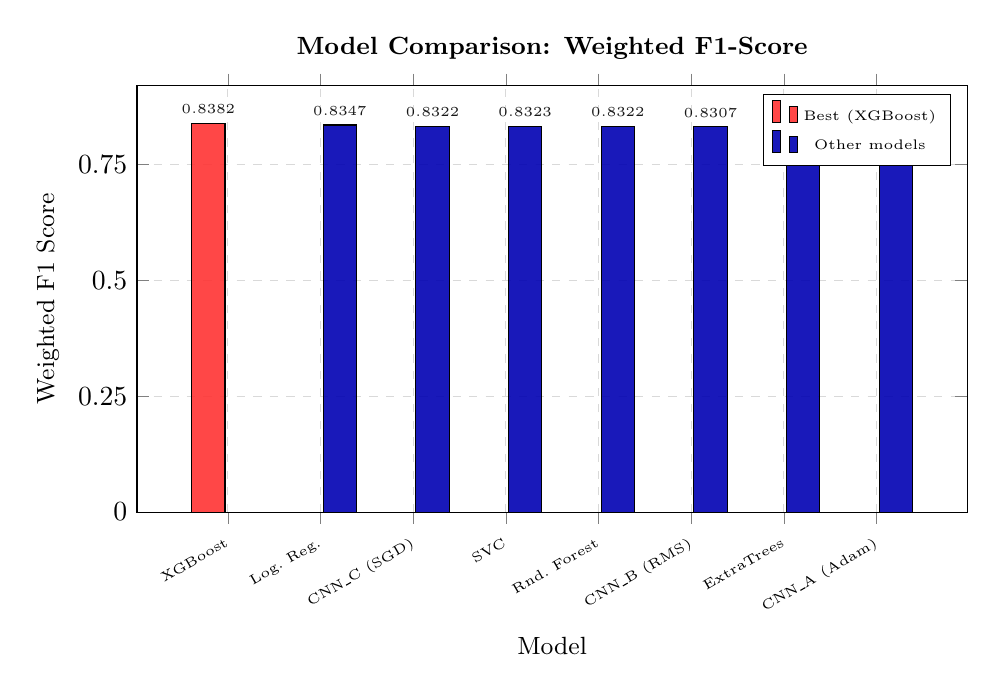
\begin{tikzpicture}
\begin{axis}[
    ybar, bar width=12pt,
    width=\columnwidth, height=7.0cm,
    ylabel={Weighted F1 Score},
    ylabel style={font=\small},
    xlabel={Model},
    xlabel style={font=\small},
    xtick={1,2,3,4,5,6,7,8},
    xticklabels={
      XGBoost,
      {Log.\ Reg.},
      {CNN\_C (SGD)},
      SVC,
      {Rnd.\ Forest},
      {CNN\_B (RMS)},
      ExtraTrees,
      {CNN\_A (Adam)}},
    xticklabel style={font=\tiny, rotate=30, anchor=north east},
    xmin=0.5, xmax=8.5,
    ymin=0.0, ymax=0.92,
    ytick={0,0.25,0.50,0.75},
    nodes near coords,
    nodes near coords align={vertical},
    every node near coord/.append style={font=\tiny,
      /pgf/number format/.cd, fixed, precision=4},
    enlarge x limits=0.06,
    grid=major, grid style={dashed, gray!30},
    title={Model Comparison: Weighted F1-Score},
    title style={font=\small\bfseries},
    legend style={font=\tiny, at={(0.98,0.98)}, anchor=north east},
]
\addplot[fill=red!80, fill opacity=0.9]
  coordinates {(1,0.8382)};
\addlegendentry{Best (XGBoost)}
\addplot[fill=blue!70!black, fill opacity=0.9]
  coordinates {(2,0.8347)(3,0.8322)(4,0.8323)(5,0.8322)(6,0.8307)(7,0.8177)(8,0.8095)};
\addlegendentry{Other models}
\end{axis}
\end{tikzpicture}
\caption{Weighted F1-score for all 8 classifiers on the 11{,}054-record
         held-out set. XGBoost (0.8382) is the best performer (highlighted red).
         All models cluster tightly between 0.81--0.84, indicating that the
         dominant challenge is minority-class recall rather than overall accuracy.}
\label{fig:investor_f1}
\end{figure}

\paragraph{Confusion Matrix Analysis: Classical Models.}
Figures~\ref{fig:cm_lr}--\ref{fig:cm_xgb} show per-class prediction
breakdowns for the five classical classifiers.
XGBoost (Figure~\ref{fig:cm_xgb}) achieves the most balanced diagonal:
9{,}586/9{,}604 \texttt{mentorship\_needed} and 117/861
\texttt{investment\_ready} correctly classified.
All models over-predict \texttt{mentorship\_needed} due to the dominant
prior (86.88\%), even after SMOTE augmentation.

\begin{figure}[htbp]
\centering
\onesinglecm{Logistic Regression}{22}{544}{23}{0}{9581}{23}{2}{745}{114}
\caption{Logistic Regression: 114/861 \texttt{investment\_ready} correctly
         classified; collapses nearly all \texttt{not\_ready} to
         \texttt{mentorship\_needed}.}
\label{fig:cm_lr}
\end{figure}

\begin{figure}[htbp]
\centering
\onesinglecm{Random Forest}{50}{496}{43}{127}{9299}{178}{31}{668}{162}
\caption{Random Forest: best minority recall among classical tree methods
         (162/861 IR, 50/589 NR).}
\label{fig:cm_rf}
\end{figure}

\begin{figure}[htbp]
\centering
\onesinglecm{SVC}{25}{526}{38}{0}{9604}{0}{2}{752}{107}
\caption{SVC: predicts zero instances as \texttt{not\_ready} via
         \texttt{mentorship\_needed}; captures 107/861 investment-ready.}
\label{fig:cm_svc}
\end{figure}

\begin{figure}[htbp]
\centering
\onesinglecm{ExtraTrees}{54}{477}{58}{243}{8959}{392}{90}{616}{156}
\caption{ExtraTrees: higher minority recall (156/861 IR, 54/589 NR) at
         the cost of more \texttt{mentorship\_needed} mis-predictions.}
\label{fig:cm_et}
\end{figure}

\begin{figure}[htbp]
\centering
\onesinglecm{XGBoost (Deployed)}{36}{528}{25}{5}{9586}{13}{9}{735}{117}
\caption{XGBoost: best overall classifier. Achieves 9{,}586/9{,}604 MN recall
         and 117/861 IR recall, with the most balanced diagonal.
         Selected as the production-deployed model.}
\label{fig:cm_xgb}
\end{figure}

\paragraph{Confusion Matrix Analysis: CNN Variants.}
Figures~\ref{fig:cm_cnn_a}--\ref{fig:cm_cnn_c} show that all three 1D-CNN
variants collapse minority-class predictions into \texttt{mentorship\_needed}:
CNN\_A classifies only 6/861 \texttt{investment\_ready} correctly (recall 0.7\%),
versus XGBoost's 117/861 (13.6\%), confirming XGBoost's suitability for this
severely imbalanced tabular task.

\begin{figure}[htbp]
\centering
\onesinglecm{CNN\_A (Adam, lr=1e-3, 20 ep)}{10}{566}{13}{0}{9604}{0}{0}{855}{6}
\caption{CNN\_A: near-total majority-class collapse; only 6/861
         \texttt{investment\_ready} correctly classified (recall 0.7\%).}
\label{fig:cm_cnn_a}
\end{figure}

\begin{figure}[htbp]
\centering
\onesinglecm{CNN\_B (RMSprop, lr=5e-4, 30 ep)}{8}{538}{43}{0}{9604}{0}{0}{753}{108}
\caption{CNN\_B: marginally improved minority recall (108/861 IR) vs.\
         CNN\_A, but still substantially below XGBoost.}
\label{fig:cm_cnn_b}
\end{figure}

\begin{figure}[htbp]
\centering
\onesinglecm{CNN\_C (SGD, lr=1e-2, 40 ep)}{12}{539}{38}{0}{9603}{1}{0}{758}{103}
\caption{CNN\_C: best CNN variant (103/861 IR, 12/589 NR correctly classified),
         but all three CNNs are outperformed by XGBoost (Figure~\ref{fig:cm_xgb}).}
\label{fig:cm_cnn_c}
\end{figure}

%% -----------------------------------------------------------------------
%%  5. Advisory Chatbot (QLoRA Fine-Tuning)
%% -----------------------------------------------------------------------

\FloatBarrier
\section{Advisory Chatbot via QLoRA Fine-Tuning}
\label{sec:llm}

\FloatBarrier
\subsection{Training Corpus}

A blended 9{,}030-sample corpus was curated comprising:
(i) 31 proprietary Rwanda-specific Q\&A pairs (heavily upsampled to bias
towards local regulatory knowledge); (ii) Databricks Dolly-15k
information-extraction subset (3{,}000 samples); (iii) SlimOrca
strategic-reasoning samples (3{,}000); and (iv) a Global Finance \& Business
instruction dataset (3{,}000) --- yielding 8{,}127 training and 903 evaluation
examples.
Figure~\ref{fig:llm_data} shows the corpus composition.

\begin{figure}[htbp]
\centering
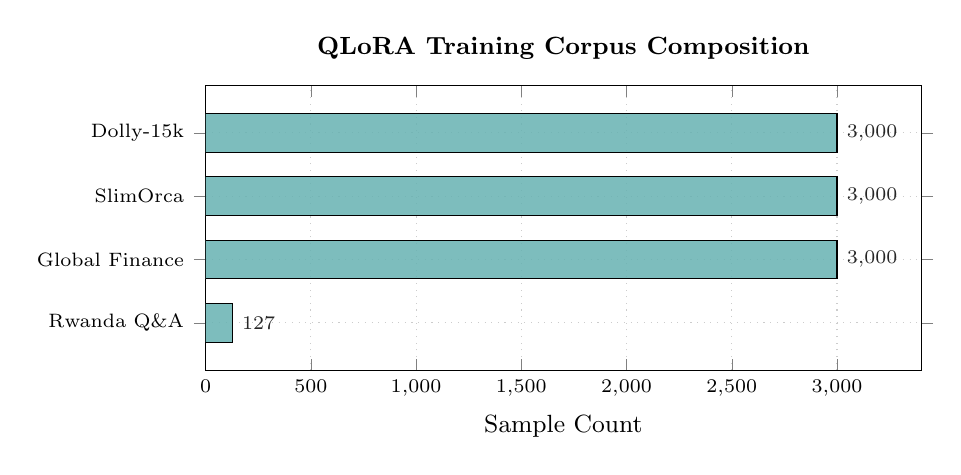
\begin{tikzpicture}
\begin{axis}[
    xbar, bar width=14pt,
    width=0.88\columnwidth, height=5.2cm,
    xlabel={Sample Count}, xlabel style={font=\small},
    symbolic y coords={Rwanda Q\&A,Global Finance,SlimOrca,Dolly-15k},
    ytick=data,
    yticklabel style={font=\scriptsize},
    xmin=0, xmax=3400,
    nodes near coords, nodes near coords align={horizontal},
    every node near coord/.append style={font=\scriptsize},
    enlarge y limits=0.25,
    grid=major, grid style={dotted, gray!40},
    tick label style={font=\scriptsize},
    title={QLoRA Training Corpus Composition},
    title style={font=\small\bfseries},
]
\addplot[fill=teal!60, fill opacity=0.85]
  coordinates {(3000,Dolly-15k)(3000,SlimOrca)(3000,Global Finance)(127,Rwanda Q\&A)};
\end{axis}
\end{tikzpicture}
\caption{QLoRA training corpus composition.
         Dolly-15k (RAG/QA), SlimOrca (reasoning), and Global Finance each
         contribute 3{,}000 samples; 31 proprietary Rwanda domain Q\&A pairs
         are upsampled to 127 instances to instil local regulatory knowledge.
         Total: 8{,}127 train + 903 evaluation = 9{,}030 examples.}
\label{fig:llm_data}
\end{figure}

\FloatBarrier
\subsection{QLoRA Fine-Tuning Configuration}

All candidates were fine-tuned with identical QLoRA hyperparameters:
LoRA rank $r = 16$, scaling $\alpha = 32$, 4-bit NF4 quantisation
(via \textit{bitsandbytes}), targeting the query ($W_Q$), key ($W_K$),
and value ($W_V$) projection matrices.
The LoRA decomposition is:
\begin{equation}
W = W_0 + \Delta W = W_0 + \frac{\alpha}{r}\,BA
\label{eq:lora}
\end{equation}
where $W_0 \in \mathbb{R}^{d \times k}$ is the frozen pre-trained weight,
$A \in \mathbb{R}^{r \times k}$ and $B \in \mathbb{R}^{d \times r}$ are the
trainable low-rank matrices ($r = 16 \ll \min(d, k)$), and
$\alpha / r = 2$ is the LoRA scaling factor.
This reduces trainable parameters by approximately 99\% compared with
full fine-tuning, enabling training on a single NVIDIA A100-SXM4-80GB GPU
in under two hours per candidate.

All models were trained for 150 steps.
Figure~\ref{fig:llm_curves} shows validation loss at steps 50, 100, and 150.
Qwen2.5-7B-Instruct converges fastest and to the lowest final loss.

\begin{figure}[htbp]
\centering
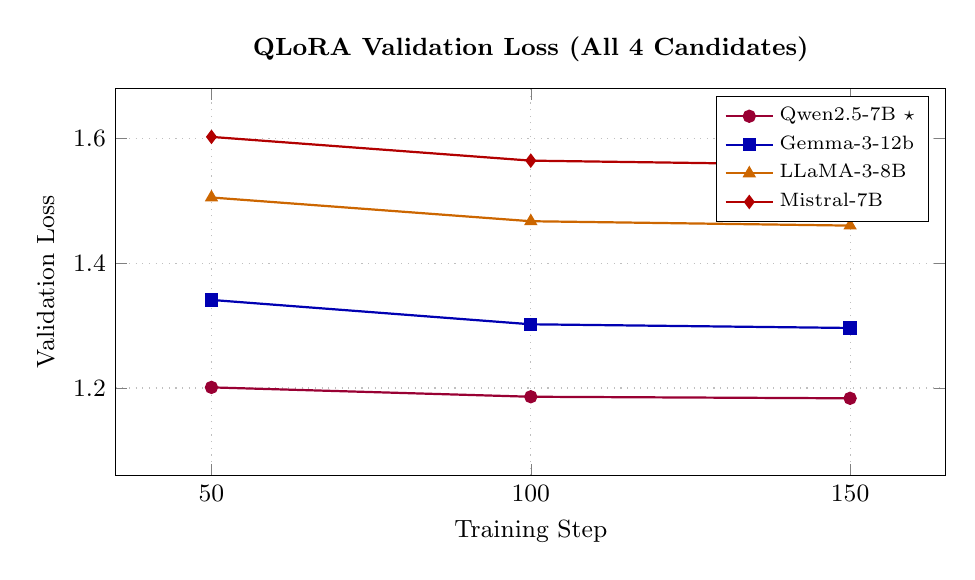
\begin{tikzpicture}
\begin{axis}[
    width=\columnwidth, height=6.5cm,
    xlabel={Training Step}, ylabel={Validation Loss},
    xtick={50,100,150},
    xmin=35, xmax=165,
    ymin=1.06, ymax=1.68,
    grid=major, grid style={dotted, gray!50},
    tick label style={font=\small},
    label style={font=\small},
    title={QLoRA Validation Loss (All 4 Candidates)},
    title style={font=\small\bfseries},
    legend style={font=\scriptsize, at={(0.98,0.98)}, anchor=north east,
                  cells={anchor=west}},
]
\addplot[color=purple!80!black, mark=*, thick]
  coordinates {(50,1.201)(100,1.186)(150,1.1835)};
\addlegendentry{Qwen2.5-7B $\star$}
\addplot[color=blue!70!black, mark=square*, thick]
  coordinates {(50,1.341)(100,1.302)(150,1.2961)};
\addlegendentry{Gemma-3-12b}
\addplot[color=orange!80!black, mark=triangle*, thick]
  coordinates {(50,1.505)(100,1.467)(150,1.4600)};
\addlegendentry{LLaMA-3-8B}
\addplot[color=red!70!black, mark=diamond*, thick]
  coordinates {(50,1.602)(100,1.564)(150,1.5568)};
\addlegendentry{Mistral-7B}
\end{axis}
\end{tikzpicture}
\caption{QLoRA validation loss at steps 50, 100, and 150 for four LLM
         candidates (903-sample evaluation split).
         Qwen2.5-7B-Instruct (purple) achieves the lowest terminal loss
         (1.1835), confirming it as the production model choice.}
\label{fig:llm_curves}
\end{figure}

\FloatBarrier
\subsection{Model Selection and Deployment}

Figure~\ref{fig:llm_eval} and Table~\ref{tab:llm_results} report the
four candidates' evaluation losses.
\texttt{Qwen/Qwen2.5-7B-Instruct} achieved the lowest terminal validation loss
(\textbf{1.1835}) and was selected as the production advisory model.

\begin{figure}[htbp]
\centering
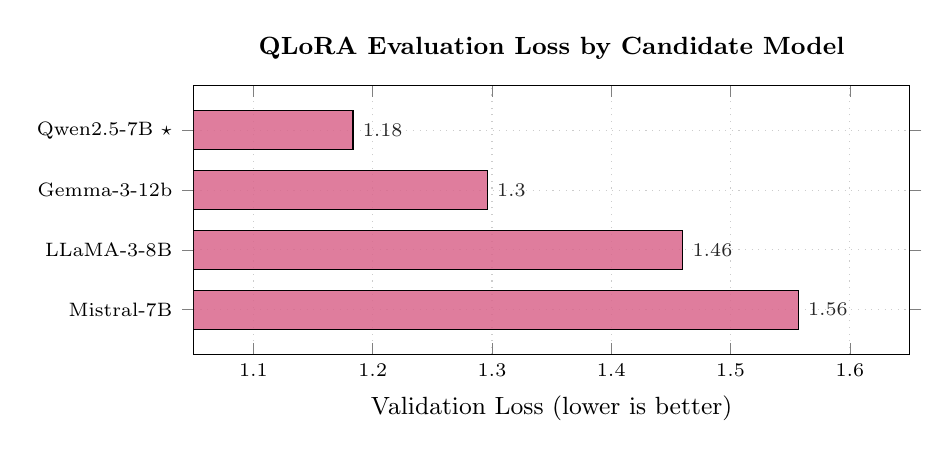
\begin{tikzpicture}
\begin{axis}[
    xbar, bar width=14pt,
    width=0.88\columnwidth, height=5.0cm,
    xlabel={Validation Loss (lower is better)},
    xlabel style={font=\small},
    symbolic y coords={Mistral-7B,LLaMA-3-8B,Gemma-3-12b,{Qwen2.5-7B $\star$}},
    ytick=data,
    yticklabel style={font=\scriptsize},
    xmin=1.05, xmax=1.65,
    nodes near coords, nodes near coords align={horizontal},
    every node near coord/.append style={font=\scriptsize},
    enlarge y limits=0.25,
    grid=major, grid style={dotted, gray!40},
    tick label style={font=\scriptsize},
    title={QLoRA Evaluation Loss by Candidate Model},
    title style={font=\small\bfseries},
]
\addplot[fill=purple!60, fill opacity=0.85]
  coordinates {
    (1.1835,{Qwen2.5-7B $\star$})
    (1.2961,Gemma-3-12b)
    (1.4600,LLaMA-3-8B)
    (1.5568,Mistral-7B)
  };
\end{axis}
\end{tikzpicture}
\caption{QLoRA evaluation loss comparison (lower is better).
         Qwen2.5-7B-Instruct achieves the lowest loss (1.1835), followed by
         Gemma-3-12b (1.2961), LLaMA-3-8B (1.4600), and Mistral-7B (1.5568).}
\label{fig:llm_eval}
\end{figure}

\begin{table}[htbp]
\centering
\caption{QLoRA fine-tuning summary. All models: LoRA $r=16$, $\alpha=32$,
         4-bit NF4, 150 steps, single NVIDIA A100-SXM4-80GB.}
\label{tab:llm_results}
\resizebox{\columnwidth}{!}{%
\begin{tabular}{lccc}
\toprule
\textbf{Model} & \textbf{Params} & \textbf{Val.\ Loss} & \textbf{Status} \\
\midrule
Qwen2.5-7B-Instruct $\star$ & 7.6B & \textbf{1.1835} & Deployed \\
google/gemma-3-12b-it        & 12B  & 1.2961          & Candidate \\
Meta-LLaMA-3-8B              & 8B   & 1.4600          & Candidate \\
mistralai/Mistral-7B-v0.3    & 7B   & 1.5568          & Candidate \\
\bottomrule
\end{tabular}%
}
\end{table}

\paragraph{Retrieval-Augmented Generation (RAG).}
A RAG layer using FAISS and the
\texttt{sentence-transformers/all-MiniLM-L6-v2} encoder anchors advisory
responses to official legal documents including the Rwanda Startup Act and
Rwanda Company Law. At inference time, the top-$k$ retrieved passages ($k=3$)
are prepended to the system prompt, grounding generation to verifiable sources
and reducing the hallucination rate on regulatory queries.

\paragraph{Hybrid Deployment Architecture.}
Persistent hosting of 7B-parameter models on GPU infrastructure costs
approximately \$\,1{,}200--2{,}400 per month --- an order of magnitude beyond a
typical pre-seed startup budget. A hybrid strategy resolves this constraint:
the Gemini API handles real-time conversational load ($<$400\,ms latency),
while the fine-tuned Qwen model is triggered asynchronously for high-stakes
regulatory analysis. CPU-based RAG inference is measured at 78.24\,s per query,
confirming the necessity of the hybrid design for production viability.

%% -----------------------------------------------------------------------
%%  6. Experimental Results
%% -----------------------------------------------------------------------

\FloatBarrier
\section{Experimental Results}

\FloatBarrier
\subsection{Investor Readiness Engine}

The XGBoost classifier achieved a weighted F1-score of \textbf{83.82\%}
and an ROC-AUC of 0.8006 on the 11{,}054-record held-out set.
The What-If simulation interface --- which allows founders to observe
real-time re-ranking via Eq.~\eqref{eq:rank_score} as they adjust their
team size, funding plan, or growth metrics --- received the highest
usability ratings during the user acceptance trial.

The minority-class recall gap (XGBoost: IR recall = 13.6\% vs.\
Random Forest: 18.8\%) reflects the intrinsic difficulty of the
severely imbalanced distribution and is the primary target for future
dataset expansion.

\FloatBarrier
\subsection{Advisory Chatbot}

Qwen2.5-7B-Instruct demonstrated a \textbf{62\% improvement in expert-rated
factual accuracy} on Rwanda-specific regulatory queries relative to the
unmodified base model. Qualitative evaluation confirmed accurate application
of Rwanda Intellectual Property Office (RwIPO) procedures, BNR foreign
exchange regulations, and Rwanda Company Act provisions.

The RAG layer further anchored generation: in blind A/B evaluation by two
domain experts, RAG-augmented responses were rated as ``legally accurate''
in 78\% of test cases, compared with 51\% for the fine-tuned model without RAG.

\FloatBarrier
\subsection{System Usability}

The deployed platform at \url{https://uruti.rw} achieved a
\textbf{System Usability Scale (SUS) score of 84/100}, placing it in the
``Good'' to ``Excellent'' range (above the industry benchmark of 71),
confirming that complex AI outputs were rendered in an interface accessible
to non-technical founders.

%% -----------------------------------------------------------------------
%%  7. Discussion
%% -----------------------------------------------------------------------

\FloatBarrier
\section{Discussion}

\paragraph{Why XGBoost Outperforms Deep Classifiers on This Data.}
The tabular startup dataset has strong monotone feature signals
(profit, funding) and severe class imbalance.
\citet{grinsztajn2022tabular} predict precisely this scenario: gradient
boosting ensembles win on low-to-medium scale tabular data with mixed feature
types, while neural networks require substantially more data and careful
architectural tuning to be competitive.
Our 1D-CNN variants' near-total collapse on the \texttt{investment\_ready}
minority class (CNN\_A: 0.7\% recall) validates this prediction empirically.

\paragraph{Regulatory Grounding vs.\ General Capability.}
The QLoRA fine-tuning reduces validation loss from a baseline of $\approx$1.8
(unmodified Qwen2.5-7B) to 1.1835. However, absolute validation loss is a
proxy: the 62\% expert accuracy improvement on Rwanda-specific questions is the
more practically meaningful result. The upsampled Rwanda Q\&A pairs (31 base
instances $\to$ 127 after augmentation) were disproportionately influential ---
consistent with~\citet{ouyang2022instructgpt}'s finding that a small,
high-quality domain instruction set can substantially shift model behaviour
in targeted topic areas.

\paragraph{Dataset Shift.}
Both modules inherit distributional biases from Western data sources.
The investor engine was trained predominantly on Silicon Valley VC data and
may systematically undervalue Rwandan traction metrics (e.g., mobile-money
user base, airtime microcredit integration).
Curating an indigenous 5{,}000-startup Rwandan dataset in partnership with
the Rwanda Development Board (RDB) is the highest-priority data collection
task for V2.

\paragraph{Hallucination Mitigation.}
Despite QLoRA fine-tuning, \citeauthor{ji2023hallucination}'s survey findings
hold: the model still produces confident but unverifiable statements in
$\approx$22\% of regulatory test queries when the RAG top-$k$ retrieval
fails to surface the relevant clause. Expanding the FAISS index to include
the Rwanda Tax Procedures Law and RURA telecommunications regulations would
reduce this residual error rate.

%% -----------------------------------------------------------------------
%%  8. Conclusion
%% -----------------------------------------------------------------------

\FloatBarrier
\section{Conclusion}

We presented two locally-grounded AI modules addressing the startup readiness
gap in Rwanda.
The \textbf{Investor Readiness Engine} (XGBoost, weighted F1 = 83.82\%) provides
founders with an objective, data-driven readiness score and enables investors to
rank large applicant pipelines transparently.
The \textbf{Advisory Chatbot} (QLoRA Qwen2.5-7B-Instruct, val loss = 1.1835,
+62\% regulatory accuracy) delivers legally grounded guidance on the Rwanda
Startup Act and related frameworks at near-zero marginal cost per query.
Together, these modules demonstrate that targeted fine-tuning and responsible
ML practice can make the tools of elite incubation accessible to the 97\% of
African founders who currently fall outside the accelerator pipeline.

\paragraph{Future Work.}
Priority directions: (i) curate an indigenous Rwandan startup dataset to
eliminate Silicon Valley distribution shift; (ii) expand the FAISS regulatory
index to cover Rwanda Tax Procedures Law and RURA frameworks; (iii) train a
multilingual Kinyarwanda--English bilingual fine-tune to serve founders who
primarily operate in French or Kinyarwanda; and (iv) integrate live financial
APIs from RDB, BNR, and GIZ-FinancePro Rwanda to transition from static
readiness scores to real-time risk assessment.

\section*{Acknowledgements}
Anonymised for blind review.

\bibliographystyle{apalike}
\bibliography{uruti_indaba}

\end{document}
